\chapter{Use-case Analysis}\label{chap:use_cases}
The introduction argued that validating properties on input parameters can become costly when data structures (such as arrays), certain data types (such as byte sequences) or a range of values have to be iterated. It showed examples for such properties and identified logical formulas containing universal quantification as amenable for distributed assertion checking. Through its domain of discourse, the quantification spans an iteration space whose elements can be checked independently by the validators. As a matter of fact, the same is also valid for existential quantification, even though its negation has a different notion than that of its universal counterpart. The difference between the two is addressed later in this chapter.

The following section formally defines a set of applicable logical formulas for the basic implementation of the distributed assertion checking scheme. \secref{sec:examples} gives some examples of such formulas. As a benchmark for the distributed scheme, the last section formalizes the cost incurred by checking formulas on Tezos in a non-distributed approach.

\section{A Set of Logical Formulas}\label{sec:formulae}
The set of formulas that can be expressed in well-formed assertions, is given in \figref{fig:formulas}. This corresponds, with some restrictions, to the language of second-order predicate logic. Besides universal and existential quantifiers (with exactly one bound variable), the definition contains logical connectives, relational symbols, constant values of a numerical, string or boolean type, variables and the functional symbols for basic arithmetic operations. This set of symbols is rather generic and should be valid for any target blockchain. Specific to the target blockchain are the sets of types $t$ and functional symbols $f$. These can only contain types and operations, which can be translated to instructions of the respective smart contract language and interpreted by the blockchain's virtual machine (VM). As an example, the primitive types in Michelson are \texttt{string}, \texttt{nat}, \texttt{int} and \texttt{bytes}, whereas Ethereum's smart contract language Solidity \cite{solidity_docs} additionally supports an \texttt{enum} type and fixed-point numbers.
\begin{align*}
    t &::= \text{primitive data types (existing in the blockchain VM)} \\
    \sigma &::= \forall \mid \exists \\
    \Theta &::= \Phi \mid \sigma (x:t) \Theta \\
    \Phi,\Psi &::= \neg\Phi \mid \Phi \Rightarrow \Psi \mid \Phi\wedge\Psi \mid
    				\Phi\vee\Psi \mid \Phi \oplus \Psi \mid M \rho N \\
    \rho &::= < \mid > \mid \le \mid \ge \mid = \mid \ne \\
    M, N &::= x \mid c \mid M \odot N  \mid f (\overline M) \\
    \odot &::= +\mid -\mid * \mid / \mid \% \\
    c &::= \text{numerical value} \mid string \mid \top \mid \bot \\
    f &::= \text{operations (existing in the blockchain VM)}
\end{align*}
\begingroup\vspace*{-\baselineskip}
\captionof{figure}{Set of logical formulas amenable to distributed assertion checking}
\label{fig:formulas}
\vspace*{\baselineskip}\endgroup

\section{Examples and Special Cases}\label{sec:examples}
This section contains a subset of use-cases that were collected in collaboration with Julian Veigl for an intermediate report \cite{bernhardt_veigel_2020}. The selection of examples covers different types and compositions of quantifiers, demonstrates different meanings of their negations, identifies special cases and discusses their implications for the implementation of distributed assertion checking.

\subsection{Two Numbers are Coprime}\label{sec:coprime}
The greatest common divisor ($gcd$) of two non-zero integers $a$ and $b$ is the largest integer that divides both evenly \cite{hardy2008introduction}. A more specific $gcd$-problem is finding two numbers which are coprime, meaning their greatest common divisor is one, i.e., $gcd(a, b) = 1$. In order to verify that two numbers are coprime, it has to be verified that there is no $gcd > 1$, hence the property of coprimeness can be expressed with the following formula in predicate logic:
\begin{equation}\label{eq:coprime-universial}
    (\forall n : int) (2 \le n \le \min(a,b)) \Rightarrow \neg((a \mathbin{\%} n) = 0 \land (b \mathbin{\%} n) = 0)
\end{equation}
Assuming it takes constant time to calculate the two remainders, checking whether two numbers satisfy this property takes linear time, i.e. $\mathcal{O}(n)$, and depends on the size of the smaller number.

When checking the assumption through a distributed effort instead, the validators consider its negation:
\begin{equation}\label{eq:coprime-existential}
    (\exists n : int) (2 \le n \le \min(a,b)) \land (a \mathbin{\%} n) = 0 \land (b \mathbin{\%} n) = 0
\end{equation}
If, within the given domain, this condition is true for a random value of $n$, the respective validator has found a counterexample.

\subsection{Heap Property}
Heaps \cite{dict_heap} are data structures based on trees and can appear in two varieties: min and max heaps. Both can be represented as binary trees and have to satisfy the heap property: in a max heap, any given node holds a value lower or equal than that of its parent, whereas in a min heap, it is greater or equal \cite{dict_heap_property}. Binary heaps are often implemented as an array, with the root of the tree stored at index 0. The relatives of a node \texttt{k} can be accessed as follows:
\begin{lstlisting}[language=Solidity, numbers=none, caption=Access a binary heap in array representation]
heap_array[(k-1)/2] // Get parent of node k
heap_array[(k*2)+1] // Get left child of node k
heap_array[(k*2)+2] // Get right child of node k
\end{lstlisting}
The min heap property for a binary heap stored in an array $a$ can be expressed in predicate logic with the following formula:
\begin{equation}\label{eq:heap-unversial}
  (\forall k : int) (1 \le k < |a|) \Rightarrow a[\lfloor(k-1)/2)\rfloor] \le a[k]
\end{equation}
The time complexity of checking whether $a$ satisfies the heap property depends on how the array is allocated. If it is dynamically sized, it takes $\mathcal{O}(n)$ in the size of the array, otherwise it takes constant time, i.e., $\mathcal{O}(1)$.  Similarly to the previous examples, counterexamples can be identified by considering the formula's negation:
\begin{equation}\label{eq:heap-unversial-neg}
  (\exists k : int) (1 \le k \le |a|) \land a[\lfloor(k-1)/2)\rfloor] > a[k]
\end{equation}

\subsection{Existential Quantification - Intersection of Sets}\label{sec:existential}
So far, this thesis only considered formulas featuring universal quantification, for which the assertion scheme engages the validators to find counterexamples. However, distributed assertion checking can not only be used to refute assumptions, but also to prove their validity. This is the case for formulas featuring existential quantification. As an example, consider the assumption that the two sets $U$ and $V$ have a non-empty intersection, i.e., $U \cap V \neq \emptyset$. If these sets are represented as arrays or lists, this property and its negation can be expressed in predicate logic by 
\begin{equation}\label{eq:intersect}
  (\exists i, \exists j) (0 \le i < |u|) \land (0 \le j < |v|) \Rightarrow u[i] = v[j]
\end{equation}
and
\begin{equation}\label{eq:intersect_neg}
  (\forall i, \forall j) (0 \le i < |u|) \land (0 \le j < |v|) \land u[i] \neq v[j]
\end{equation}
Due to the universal quantifiers in the negation, finding random values for $i$ and $j$ for which the condition $u[i] \neq v[j]$ is valid does not produce a counterexample. If the condition is false, however, it produces a proof for the validity of the assumption, as it identified an element that is present in both sets. In that case, the validator finding such a proof should publish an approval instead of a veto to the network. After an approval has been posted, and all validators have come to a consensus about the validity of the proof, the result is accepted. For the blockchain protocol, this implies that distributed refutation and validation have to be implemented as separate modi of assertion checking.

Concerning the complexity of this assertion, the property can be checked in $\mathcal{O}(|u|*|v|)$. By considering the cardinality of their union $n = |u|+|v|$, one can derive that the worst case occurs when both sets have the same size, i.e., $|u| = |v| = n/2$. This leads to a quadratic complexity $\mathcal{O}(n/2 * n/2) = \mathcal{O}(n^2/4) = \mathcal{O}(n^2)$.

\subsection{Nested Quantification - SAT Problems}
The previous example demonstrated that universal and existential quantification have to be handled differently. However, further special cases, caused by nested quantification, have to be considered as well. A nesting of the same type of quantifier, e.g. $\forall i \forall j$, can be considered as trivial. They can be translated to code generating a random value for each predicate variable and checking for a counterexample or proof respectively. It becomes less trivial, if the nesting contains both universal and existential quantifiers. This section examines the cases of $\forall i \exists j$ and $\exists i \forall j$ on the basis of a contract that expects a solution for a boolean satisfiability problem (SAT).

Instances of SAT problems consist of a formula $F$ in propositional logic, and determine if there exists a variable assignment $\mathcal{A}$ to the values $true$ or $false$, s.t. the formula is satisfied ($\mathcal{A}(F) = 1$) \cite{Biere2009}. Modern SAT-solvers expect $F$ to be in conjunctive normal form (CNF), i.e., a conjunction of a set of clauses, where clauses are disjunctions of variables or their negations (called literals) \cite{cnf_math_encycl}. While finding an assignment $\mathcal{A}$ that satisfies $F$ is a NP-complete problem, verifying whether a given assignment satisfies the formula takes $\mathcal{O}(n*m)$, where $n$ is the number of clauses and $m$ the number of variables (in the worst case, every variable is present as a literal in each clause). In the case of k-SAT problems, where each clause contains at most k literals, the complexity is reduced to $\mathcal{O}(n)$.

\subsubsection{Encoding of Variables, Literals and Clauses}
A SAT problem can be represented as a list of clauses $c$ and a variable assignment $\mathcal{A}$. To avoid having to handle the variables and their literals as strings, and thus optimize runtime and memory consumption, the following uses an encoding scheme \cite{sabablog}.

Variables are encoded by a unique number starting from $0$ to $n-1$, where $n$ is the total number of variables. The positive and negative literals of a variable with id $x$ are encoded by the function
\begin{align*}
encode(x) =
\begin{cases}
  $2x$  & \text{if x is present as a positive literal}\\
  $2x+1$ & \text{if x is present as a negated literal}\\
\end{cases}   
\end{align*}
Consequently, checking whether a literal $y$ is positive or negative is a simple bit-wise $AND$ operation:
\begin{align*}
\texttt{isPositive(y) = y \& 1 == 0}
\end{align*}
Consider the following boolean formula and variable assignment:
\begin{align*}
F = (A \vee B) \wedge (B \vee \neg C) \text{, } \mathcal{A} = \{A \rightarrow false, B \rightarrow true, C \rightarrow false\}
\end{align*}
Following the encoding of variables given above, the list of variables $v=[A,B,C]$ occurring in $F$ is encoded as $v_{enc} = [0,1,2]$. If clauses are given as lists of literals, $F$ can be represented by the encoding $F_{enc} = [[0,2],[2,5]]$. Since the encoding of variables corresponds to their index in the list of variables, $\mathcal{A}$ can be passed as a list of booleans that maintains the same order of variables: $\mathcal{A}_{enc} = [False, True, False]$. If the blockchain's VM supports a respective data type, $\mathcal{A}$ can alternatively be represented with a more efficient bitarray. Lastly, the variable encoding $x$ of a literal $y$ is obtained by dividing its encoding by two, which corresponds to a bit-wise shift to the right:
\begin{align*}
\texttt{decode(y) = y >> 1}
\end{align*}

\subsubsection{Satisfiability in Predicate Logic - CNF}
Consider a contract that expects a SAT problem in CNF and a proposed assignment, both encoded as described above. Assuming that $F$ is a k-SAT instance, the assumption that $\mathcal{A}$ satisfies $F$ can be expressed in predicate logic as follows:
\begin{equation}\label{eq:cnf_sat}
\begin{aligned}
(\forall i : int, \exists j : int) &(0 \leq i < |F|) \wedge (0 \leq j < k) \\
&\Rightarrow ((isPositive(F[i][j]) \wedge \mathcal{A}[decode(F[i][j])]) \\
&\vee (\neg isPositive(F[i][j]) \wedge \neg \mathcal{A}[decode(F[i][j])])))
\end{aligned}
\end{equation}

In the previous examples, where formulas contained only a single quantifier, the predicate variables of the negated formula are replaced by a randomly generated number during assertion checking. Quantifiers thus are translated to random generators during the generation of target code. However, by checking a random literal in a random clause, the validator cannot make a definite statement about whether $\mathcal{A}$ satisfies $F$. Each clause has to be examined as a whole in order to verify that the conjunction evaluates to true. Consequently, the distribution can only take place on the level of clauses, but not on the level of literals. Each validator thus has to check all literals of one random clause, which translates into a random generator for the universal quantifier, and a loop for the existential quantifier. Whether the assertion requires a proof or a counterexample can be derived from the outer quantifier, hence validators produce a counterexample in this case. \lstref{lst:cnf_test_code} shows the generated testing code of the CNF SAT problem, where \texttt{check} evaluates the negated condition. While formulas with a single quantifier simply translate to generating a random value and checking the condition, this code is more extensive. It requires a more sophisticated compiler, which can differentiate between different quantification compositions.

\begin{lstlisting}[label=lst:cnf_test_code, caption=Test code structure for single nested quantifiers, numbers=none]
i = random(0, size(F))
for (j : [0..k)):
  if not check( ... ):
    // property holds
    return true
// counterexample found
return false
\end{lstlisting}

Due to the loop, the cost incurred by one validator checking the assertion becomes, in the worst case, linear in the number of literals in the clause. An exception is the case of k-SAT instances, where the cost per validators remains constant, albeit with a factor $k$. 

\subsubsection{Satisfiability in Predicate logic - DNF}\label{sec:dnf}
The same propositional formula with the reversed quantification nesting $\exists i \forall j$, describes the assertion for the assumption $\mathcal{A}(F) = 1$, where $F$ is given in disjunctive normal form (DNF), i.e., a disjunction of conjunctions \cite{dnf_math_encycl}:
\begin{equation}\label{eq:dnf_sat}
\begin{aligned}
(\exists i : int, \forall j : int) \: &(0 \leq i < |F|) \wedge (0 \leq j < k) \\
&\Rightarrow ((isPositive(F[i][j]) \wedge \mathcal{A}[decode(F[i][j])]) \\
&\vee (\neg isPositive(F[i][j]) \wedge \neg \mathcal{A}[decode(F[i][j])])))
\end{aligned}
\end{equation}
The translation to code can be approached in the same way than its CNF counterpart. Instead of a counterexample, this use-case demands for a proof.

\subsection{Further Nesting}
Nesting is, of course, not limited to two quantifiers. Generally, formulas containing universal or existential quantification exclusively within the nesting benefit the most from distributed assertion checking, as each quantifier can be translated into a random generator. On the other hand, formulas with both types and a transition from one to the other early in the order benefit the least; starting from the first transition, the subsequent quantifiers are translated to loops.

To substantiate this argument, consider two variations of a contract that expect a list of boolean formulas in CNF, and an assignment $\mathcal{A}$. Variation 1 checks, whether $\mathcal{A}$ satisfies at least one $F$. Variation 2 checks, if all $F$ are satisfied. This can be expressed by nesting quantifiers as follows: 
\begin{enumerate}
\item $\forall f \forall i \exists j$
\item $\exists f \forall i \exists j$
\end{enumerate}
In the first case, each validator picks a random clause from a random $F$, and checks if at least one literal evaluates to true. This translates to two random generators and a loop for the existential quantifier. In the second case, checking a random clause in isolation cannot prove the satisfiability, hence the validator has to check all clauses in a loop. This translates to one random generator and two loops. The same reasoning can be done for the reverse order, i.e. $\exists\exists\forall$ and $\forall\exists\forall$.

\section{Restriction of Use-cases}\label{sec:restrict}
The examples given in this chapter have shown that, depending on the type and order of quantification, not all properties can be checked in the same way and need different modi of assertion checking. Additionally, they require a distinct translation to target code. This increases the complexity and requirements for an implementation of the toolchain and protocol amendment; therefore, as a first iteration, this thesis focuses on providing a design and toolchain for assertions using universal quantification only.

\section{Cost Analysis of a Local Approach}\label{sec:usecase_cost}
For the purpose of having a benchmark for the evaluation of the distributed approach, this section analyses the cost of invoking a contract on the blockchain which checks a formula locally. Given that the target blockchain is Tezos, the computational and storage-related costs of a transaction are represented in units of gas. Although they are not paid directly in terms of fees, the actual fees paid to the miner (called bakers in Tezos) are based on the gas consumption. The gas model of Tezos is described in more detail in \secref{sec:tezos}. According to this model, the total gas consumption of a transaction $T(source,\, destination=C,\, arg, \, ...)$ invoking a smart contract $C(storage, \, parameter\, type, \, code)$ is calculated by \eqref{eq:gas_transaction}, where $I$ is the set of internal operations:
\begin{align}\label{eq:gas_transaction}
\begin{split}
GasConsumed(T) = \quad &base \, gas \, cost \\
+& \, gasRead(code) \\
+& \, gasRead(storage) \\
+& \, gasDeserialize(storage, \, arg) \\
+& \, gasParseType(parameter \, type, \, storage) \\
+& \, gasParseData(storage, \, arg) \\
+& \, gasParseCode(code) \\
+& \, gasInterpret(code, \, arg, \, storage) \\
+& \, gasUnparse(storage) \\
+& \, gasSerialize(storage) \\
+& \, gasWrite(storage) \\
+& \, \sum_{i \in I} GasConsumed(i)
\end{split}
\end{align}
Assuming the storage of the contract is never increased, the amount of gas returned by the cost functions independent of the argument, i.e., the parameter value, remains constant for each $T$. The cost functions for the deserialization, parsing and interpretation, however, are functions of $arg$ and grow monotonically with increasing sizes of $arg$ \cite{morley_gasmodel}\cite{tezos_repo}.

Consider the following simple contracts --- they do not do anything useful, but can be used to approximate the amplification of costs with regard to $arg$. Function \texttt{foo} of contract \texttt{Foo} takes an integer as input parameter, whose byte sequence representation does not increase significantly with higher values. Thus, the increase in overall costs is mainly accounted for by the interpretation cost. Contract \texttt{Bar}, on the other hand, executes similar operations as function \texttt{foo} in function \texttt{bar}, but expects a list of integers instead. The list data type uses notably more memory with increasing input sized and thus causes higher deserialization and parsing costs on top of the interpretation cost. 
\begin{lstlisting}[numbers=none, language=Solidity, caption=Simple dummy contract expecting an integer and executing a loop]
contract Foo {
  function foo (int a) public {
    for (uint i = 0; i < a; i++) {
      assert(a == a)
    }
  }
}
\end{lstlisting}
\begin{lstlisting}[numbers=none, language=Solidity, caption=Simple dummy contract expecting iterating over a list]
contract Bar {
  function bar (int [] b) public {
    for (uint i = 0; i < b.length; i++) {
      assert(b[i] = b[i])
    }
  }
}
\end{lstlisting}

\figref{fig:use_case_cost} shows the reported gas consumption of transactions calling the corresponding dummy contracts implemented in Michelson (cf. Appendix \ref{apx:cost_analysis_contract}) on the Delphinet test network \footnote{\url{https://tezos.gitlab.io/introduction/test_networks.html\#delphinet}}. As to be expected, the gradient of the cost function in the case of \texttt{Bar.bar} is higher due to additional serialization and parsing costs, namely $\frac{dx}{dy} = 16$ compared to $\frac{dx}{dy} = 6$ for \texttt{Foo.foo}.
\begin{figure}[h]
\centering
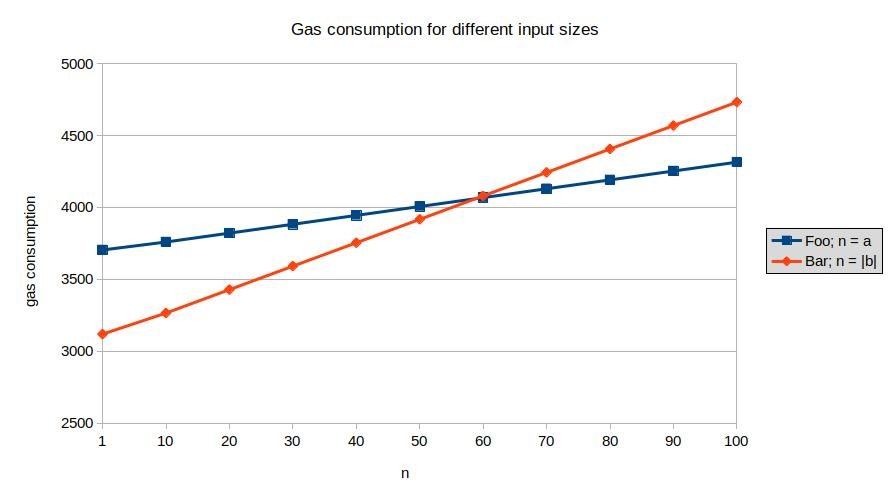
\includegraphics[width=0.9\linewidth]{figures/2-use_cases/cost_analysis}
\caption{Gas consumption of contracts \texttt{Foo} and \texttt{Bar} for increasing input sizes}
\label{fig:use_case_cost}
\vspace{128in}
\end{figure}

Besides inflicting higher transaction costs on the user with increasing parameter sizes, a local approach also causes a higher ``footprint'' on the blockchain network. The transaction has to be processed at every full node of the network, which do not get any rewards in return (except for the nodes that were assigned baking or endorsement rights for the current block\footnote{Tezos' Proof of Stake consensus mechanism is described in \secref{sec:tezos}}).
